\documentclass{article}
\usepackage[utf8]{inputenc}
\usepackage[margin=1.25in]{geometry}
\usepackage{amsmath}
\usepackage{graphicx}
\usepackage{wrapfig}
\let\vec\mathbf
\usepackage{listings}
\usepackage{color}
\usepackage{amsmath}
\usepackage{graphicx}
\usepackage{wrapfig}

\definecolor{dkgreen}{rgb}{0,0.6,0}
\definecolor{gray}{rgb}{0.5,0.5,0.5}
\definecolor{mauve}{rgb}{0.58,0,0.82}

\lstset{frame=tb,
  language=Python,
  aboveskip=3mm,
  belowskip=3mm,
  showstringspaces=false,
  columns=flexible,
  basicstyle={\small\ttfamily},
  numbers=none,
  numberstyle=\tiny\color{gray},
  keywordstyle=\color{blue},
  commentstyle=\color{dkgreen},
  stringstyle=\color{mauve},
  breaklines=true,
  breakatwhitespace=true,
  tabsize=3
}



\title{Intro to OpenCV}
\author{ Neal Bayya, George Tang }
\date{September 2018}

\begin{document}

\maketitle

\section{Introduction}
OpenCV provides a very powerful framework for projects involving images and videos. It provides low-level computer vision functions, such as masking, blurring, and transforming images, edge detection, and basic image segmentation, as well as a statistical machine learning library (Decision trees, KNN, SVMs). OpenCV is compatible with multiple programming languages, and multiple platforms, including Numpy, Tensorflow, Keras, and PyTorch.

\section{Tensors}
The tensor is the fundamental building block of OpenCV and many other platforms, hence why OpenCV can be robustly integrated with them.

A tensor is defined as multi-dimensional geometric object, where each dimension is represented by a vector. The vectors are recursive, meaning the components of the first vector are vectors that represent the second dimension, and so on. For instance, imagine you have a dataset composed of 2000 128x128 pxl RGB images. The tensor would have shape of (2000, 128, 128, 3). 

Math on tensors are recursively vectorized, meaning that the first dimension of the tensors are processed just like regular vectors, and the process repeats on the second dimension. For instance, lets say I want to add two 2 by 2 tensors. 

\[
\begin{bmatrix}
[ 2 & 3 ] \\
[ 3 & 5 ]
\end{bmatrix}
=
\begin{bmatrix}
[ 1 & 0 ]\\
[ 0 & 1 ] 
\end{bmatrix}
+
\begin{bmatrix}
[ 1 & 3 ] \\
[ 3 & 4 ]
\end{bmatrix}
\]

\noindent
Subtraction, matrix multiplication, dot project, etc. can be generalized in such a way. This branch of mathematics is know as tensor calculus. Numpy provides robust implementations of these operations. The code for the above example would look like. 

\begin{lstlisting}
import numpy as np

a = np.array([[1, 0], [0, 1]])
b = np.array([[1, 3], [3, 4]])
c = a+b
print(c)

>> [[2, 3], [3, 5]]
\end{lstlisting}

\section{Getting Started with Images}
For our first project, we will learn read and save (write) images. Images are read and written as tensors. cv.waitKey(0) closes the frame window when the user presses the enter key. The 0 means wait indefinitely. If there is a value, then it is the maximum time in milliseconds the frame will show. 

\begin{lstlisting}
import cv2 as cv

img = cv.imread('input.jpg')
cv.imshow('Framename', img)
cv.waitKey(0)
cv.imwrite('Filename', img)

\end{lstlisting}

\section{Low-Level Image Processing}
OpenCV provides documentation and mathematical tools for image processing. Now, we will go over these particular OpenCV functions.  

\subsection{Geometric Transformations}
Last lecture, we learned about transformations such as rotation, translation, and perspective transform.  With OpenCV, we can perform these operations and also identify the transformation matrix for two corresponding images.

\begin{itemize}
    \item \textbf{cv2.warpAffine(src, M, dsize)} can be used to transform a given image (src) using the 2x3 transformation matrix (M) to an output image of a specified size (dsize).  It is important to note that OpenCV provides functions for finding the rotation transformation matrix given a specified angle (\textbf{cv2.getRotationMatrix2D}) and performing the scaling affine transformation (\textbf{cv2.resize()}).  
    
    \item The \textbf{cv2.warpPerspective(src, M, dsize)} function applies a perspective transformation to the image. As we learned last week, this function is performed with a 3x3 transformation matrix.
\end{itemize}
\noindent
Given input and output points, we can ask OpenCV to fit a particular transformation matrix to it.  \textbf{cv2.getAffineTransform(pts1, pts2)} can give you a 2x3 matrix that transforms pts1 to pts2, where pts1 and pts2 contain the corresponding points on the image.  


Consider the following problem: We have an image of a sudoku puzzle but much of the filler newspaper is included in the image.  On top of that, the image was taken at an angle.  We can use the OpenCV to transforming the corners of the sudoku puzzle to the corners of the image.  Refer to Figure \ref{Sudoku} for clarity.

\begin{figure}[!htbp]
\begin{center}
   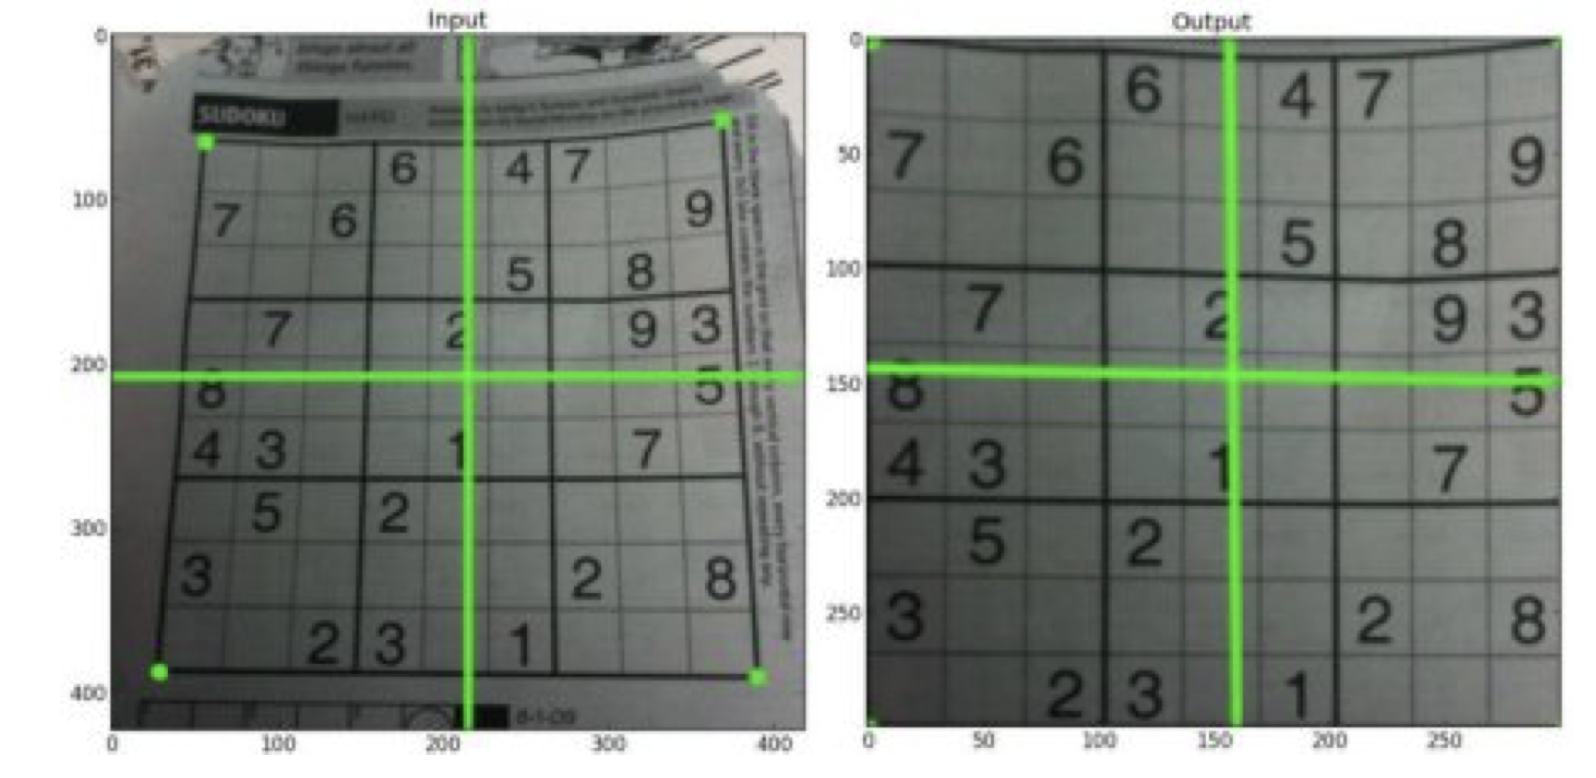
\includegraphics[width=8cm]{sudoku.png} 
   \caption{Sudoku Perspective Transform}
   \label{Sudoku}
\end{center}
\end{figure}
\noindent
Demo code is shown below for modeling a perspective transform from the puzzle corners to the image corners.  This perspective transform is then applied to the image.
\begin{lstlisting}
img = cv2.imread('sudokusmall.png')
rows,cols,ch = img.shape

#Pts1 identifies coordinates of the sodoku puzzle corners
#Pts2 identifies the coordinates of where we want pts1 to transform to (ie image corners)
pts1 = np.float32([[56,65],[368,52],[28,387],[389,390]])
pts2 = np.float32([[0,0],[300,0],[0,300],[300,300]])

#model pts1->pts2 with transform matrix
M = cv2.getPerspectiveTransform(pts1,pts2)
#apply the transformation to the whole image and plot
dst = cv2.warpPerspective(img,M,(300,300))
plt.subplot(121),plt.imshow(img),plt.title('Input')
plt.subplot(122),plt.imshow(dst),plt.title('Output')
plt.show()
\end{lstlisting}

\subsection{Blurs and Filters}

\begin{itemize}
    \item \textbf{cv2.filter2D()} is an OpenCV function that can be used for convoluting an image with a given kernel.  For example, you can bring an image to lower resolution by using an averaging kernel.  For example, 
    \begin{bmatrix}
    $0.25 & 0.25  \\
    0.25 & 0.25$
    \end{bmatrix}
    can be passed and convolved along 2x2 patches in the image.  You can think of convolution as taking a dot product of the kernel values and the image patch. The resulting image have half the size in width and height. 

    \item Averaging kernels are typically not used to blur images because they keep noise in the image.  Gaussian filtering can be used instead, where the kernel models a two-dimensional kernel function rather than a constant average.  The Gaussian function is $G(x) = \frac{1}{\sqrt{2\pi\sigma^2}}e^{-\frac{x^2}{2\sigma^2}}$ The Gaussian kernel can be created with various sizes using the  \textbf{cv2.getGaussianKernel()} function.  
\end{itemize}

\section{Videos}
Videos are composed on images, called frames. The FPS of a video is frames/second. Below is some sample code that records video from the camera, displays it, and saves it.

\begin{lstlisting}
cap = cv.VideoCapture(0)
fourcc = cv.VideoWriter_fourcc(*'XVID')
out = cv.VideoWriter('output.avi', fourcc, 20.0, (640,480))
frames = 200 #play and save 200 frames
cnt = 0
while(True):
    if (cnt == 200) break
    ret, frame = cap.read() # Capture frame-by-frame
    cv.imshow('frame',gray) # Display the resulting frame
    out.write(frame)
    cnt+=1
cap.release()
out.release()
\end{lstlisting}

\end{document}

